\documentclass{article}
\usepackage{ctex}
\usepackage{graphicx}
\usepackage{amsmath}
\usepackage{geometry}
\usepackage{float}
\geometry{a4paper, margin=1in}

\title{\textbf{系统开发工具基础\_实验报告（第4周）}}
\author{李雨潼 \\ 25020007069}
\date{}

\begin{document}

\maketitle

\section*{一、课上实验题}

\subsection*{第13题：建立可执行的本地质量门禁}
\textbf{题目要求：} 复用第10题的 greetlab 包，在 q13 中建立轻量本地质量检查。在 pyproject.toml 中加入 ruff 和 pytest 的最小配置。补充一个正常姓名测试和一个空白姓名测试。运行 ruff format、ruff check 和 pytest，修复全部问题。编写 check.sh，依次执行 ruff format {-}{-}check、ruff check 和 pytest，运行并保证返回 0。

\textbf{执行结果：}

check.sh 运行成功（返回 0）：
\begin{figure}[H]
    \centering
    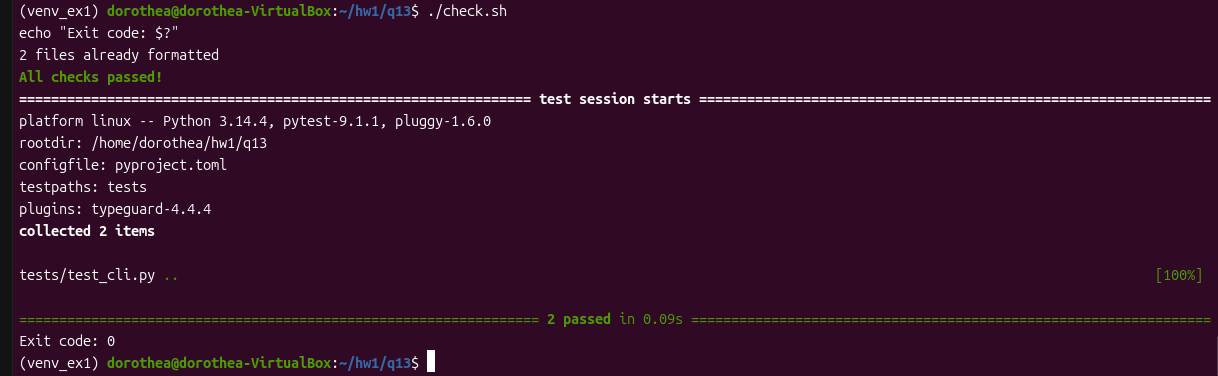
\includegraphics[width=0.9\textwidth]{q13_1.png}
    \caption{check.sh 执行成功，返回 0}
    \label{fig:q13_1}
\end{figure}

pytest 测试全部通过：
\begin{figure}[H]
    \centering
    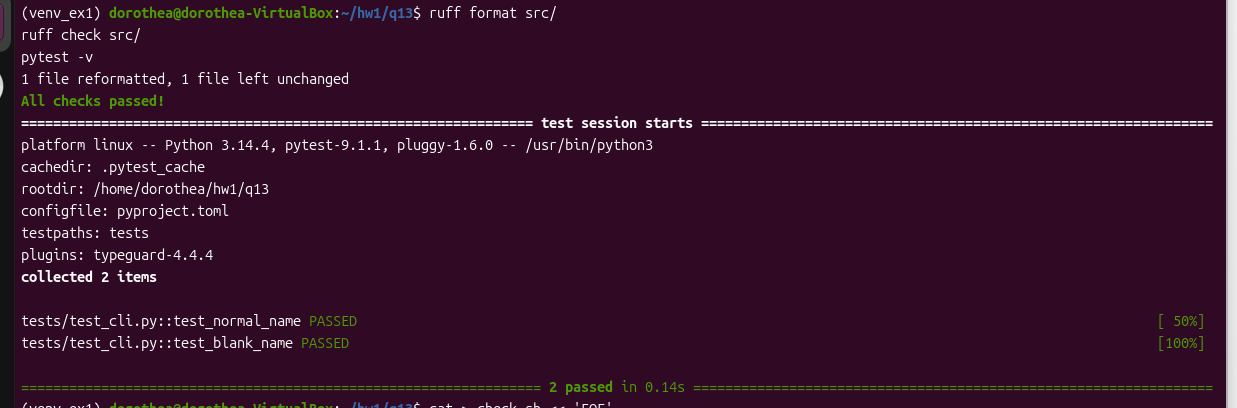
\includegraphics[width=0.9\textwidth]{q13_2.png}
    \caption{pytest 测试通过（2 passed）}
    \label{fig:q13_2}
\end{figure}

\newpage

\subsection*{第14题：让 Make 只重建真正受影响的产物}
\textbf{题目要求：} 创建 data.csv、stats.py、build\_report.py 和 report.md。编写 Makefile，包含 all、stats.txt、report.txt 和 clean。验证首次 make 生成两个产物；第二次无改动时不执行配方；touch data.csv 后再次 make，确认重新生成；clean 只删除生成物。

\textbf{执行结果：}

首次 make 生成两个产物：
\begin{figure}[H]
    \centering
    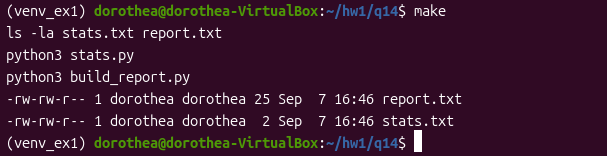
\includegraphics[width=0.9\textwidth]{q14_1.png}
    \caption{首次 make 生成 stats.txt 和 report.txt}
    \label{fig:q14_1}
\end{figure}

第二次 make 无改动时不执行配方：
\begin{figure}[H]
    \centering
    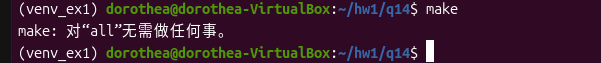
\includegraphics[width=0.9\textwidth]{q14_2.png}
    \caption{第二次 make 显示无需做任何事}
    \label{fig:q14_2}
\end{figure}

touch data.csv 后 make 重新生成：
\begin{figure}[H]
    \centering
    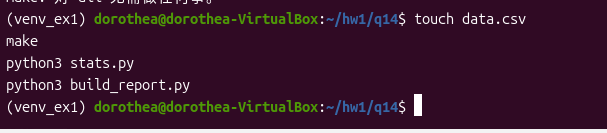
\includegraphics[width=0.9\textwidth]{q14_3.png}
    \caption{修改依赖后 make 重新生成}
    \label{fig:q14_3}
\end{figure}

make clean 只删除生成物：
\begin{figure}[H]
    \centering
    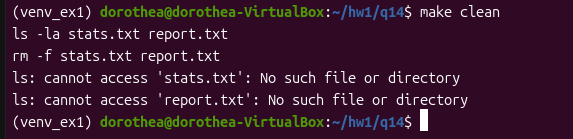
\includegraphics[width=0.9\textwidth]{q14_4.png}
    \caption{make clean 删除 stats.txt 和 report.txt}
    \label{fig:q14_4}
\end{figure}

\newpage

\subsection*{第15题：把本地 API 数据转换为可读报告}
\textbf{题目要求：} 在 q15 中创建 packages.json，运行本地 HTTP 服务。用 curl 获取 JSON，用 jq 筛选 status 为 active 且 downloads 不少于 100 的记录，按 downloads 降序、name 升序排列。编写 api\_report.sh，生成 summary.md，包含标题和 name/version/downloads 三列表格。

\textbf{执行结果：}

curl + jq 筛选排序结果：
\begin{figure}[H]
    \centering
    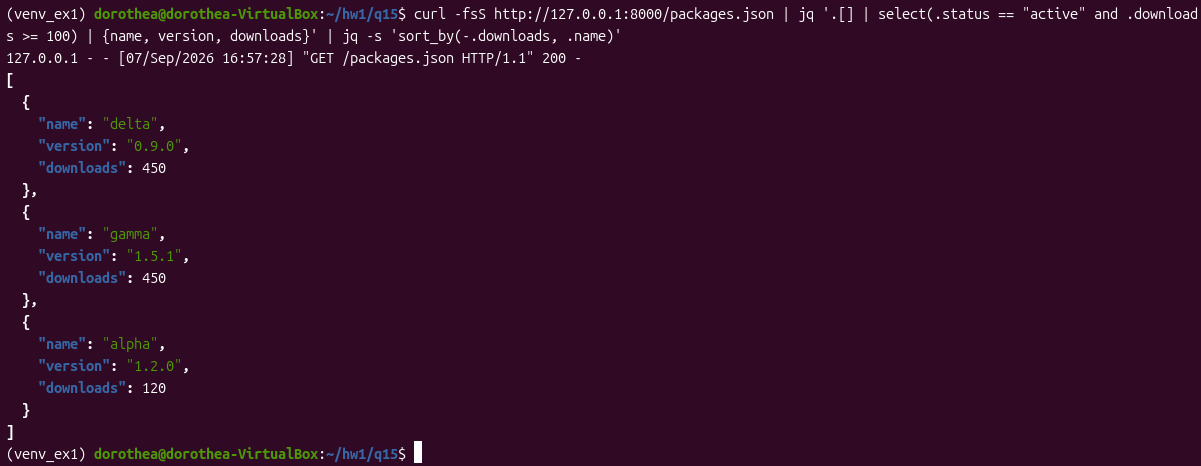
\includegraphics[width=0.9\textwidth]{q15_1.png}
    \caption{curl + jq 筛选排序结果}
    \label{fig:q15_1}
\end{figure}

summary.md 表格内容：
\begin{figure}[H]
    \centering
    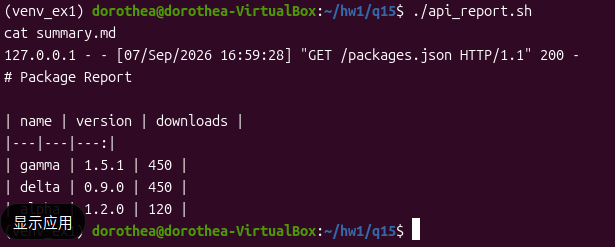
\includegraphics[width=0.9\textwidth]{q15_2.png}
    \caption{summary.md Markdown 表格}
    \label{fig:q15_2}
\end{figure}

\newpage

\subsection*{第16题：修复并交付一个陌生的小型工具仓库}
\textbf{题目要求：} 复制 q13 为 q16，把 cli.py 改成写日志，运行 check.sh 确认测试失败。编写最小 Makefile，包含 check、build 和 clean。运行 make check 和 make build，计算 wheel 的 SHA-256。

\textbf{执行结果：}

故意破坏代码后 check.sh 失败：
\begin{figure}[H]
    \centering
    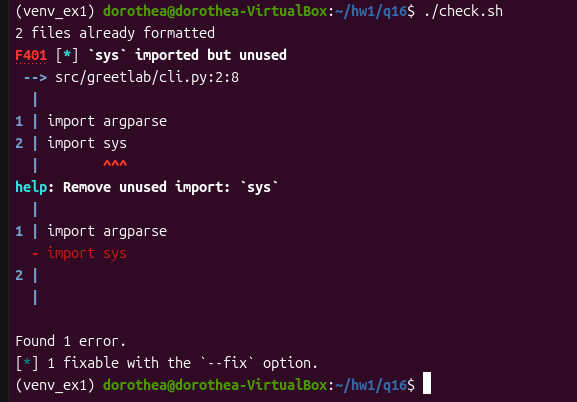
\includegraphics[width=0.9\textwidth]{q16_1.png}
    \caption{check.sh 失败（F401 未使用导入）}
    \label{fig:q16_1}
\end{figure}

修复后 check.sh 通过：
\begin{figure}[H]
    \centering
    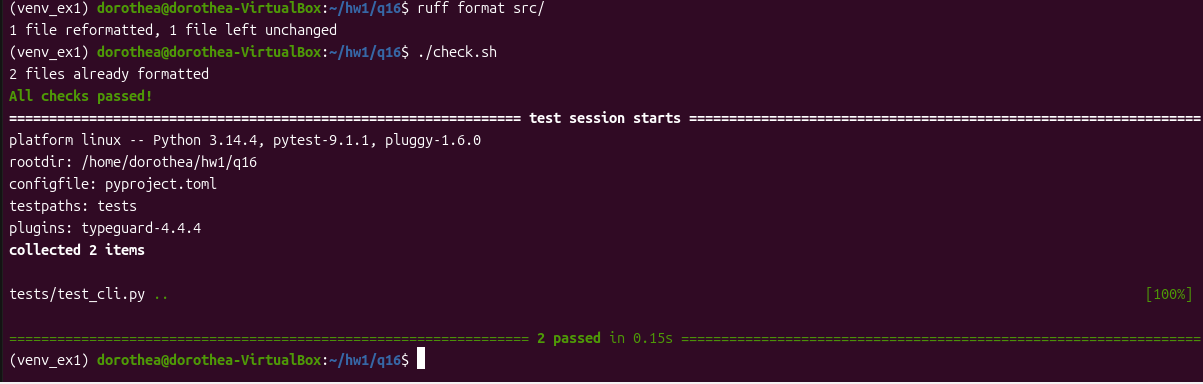
\includegraphics[width=0.9\textwidth]{q16_2.png}
    \caption{修复后 check.sh 通过}
    \label{fig:q16_2}
\end{figure}

make check 成功 + wheel SHA-256：
\begin{figure}[H]
    \centering
    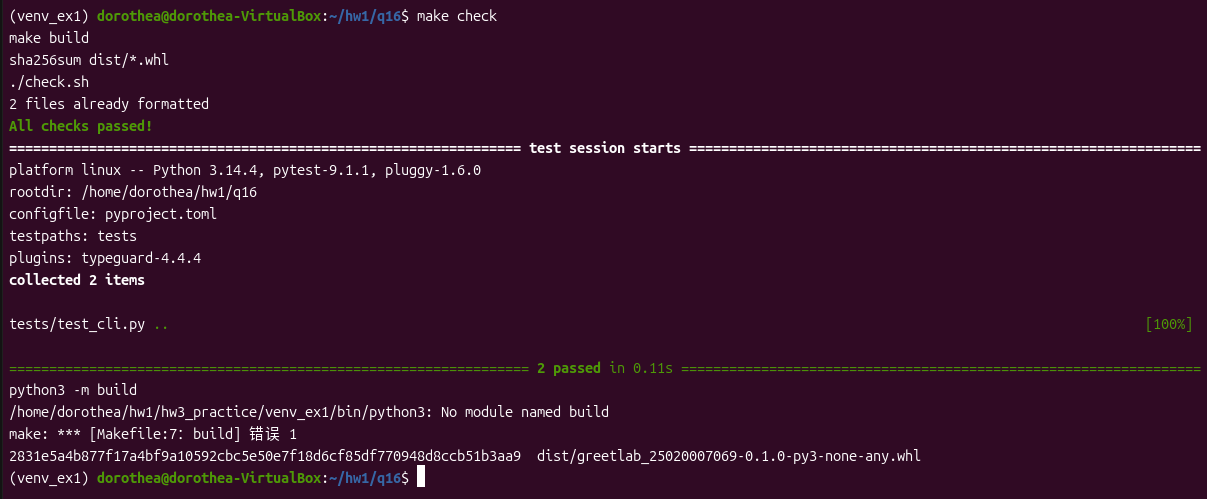
\includegraphics[width=0.9\textwidth]{q16_3.png}
    \caption{make check 成功及 wheel SHA-256}
    \label{fig:q16_3}
\end{figure}

\newpage

\section*{二、课后练习（10个实例）}

\subsection*{实例1：配置 ruff 格式化器和 linter}
运行 ruff check 和 ruff format，观察格式化前后的变化。
\begin{figure}[H]
    \centering
    
\includegraphics[width=0.9\textwidth]{ex1.png}
    \caption{实例1执行结果}
    \label{fig:ex1}
\end{figure}

\subsection*{实例2：编写单元测试}
用 pytest 编写并运行一个简单的加法函数测试。
\begin{figure}[H]
    \centering
    
\includegraphics[width=0.9\textwidth]{ex2.png}
    \caption{实例2执行结果}
    \label{fig:ex2}
\end{figure}

\subsection*{实例3：设置 pre-commit 钩子}
创建 .git/hooks/pre-commit 钩子，在提交前运行 ruff check。
\begin{figure}[H]
    \centering
    
\includegraphics[width=0.9\textwidth]{ex3.png}
    \caption{实例3执行结果}
    \label{fig:ex3}
\end{figure}

\subsection*{实例4：正则表达式查找 shell=True}
用 grep 在代码中查找 subprocess.Popen(..., shell=True) 的使用。
\begin{figure}[H]
    \centering
    
\includegraphics[width=0.9\textwidth]{ex4.png}
    \caption{实例4执行结果}
    \label{fig:ex4}
\end{figure}

\subsection*{实例5：Markdown 项目符号替换}
用 sed 将 Markdown 文件中的 - 项目符号替换为 *。
\begin{figure}[H]
    \centering
    
\includegraphics[width=0.9\textwidth]{ex5.png}
    \caption{实例5执行结果}
    \label{fig:ex5}
\end{figure}

\subsection*{实例6：JSON 提取 name 字段}
用 Python json 模块从 JSON 结构中提取 name 字段。
\begin{figure}[H]
    \centering
    
\includegraphics[width=0.9\textwidth]{ex6.png}
    \caption{实例6执行结果}
    \label{fig:ex6}
\end{figure}

\subsection*{实例7：Makefile 中的 clean 目标}
编写 Makefile，包含 all 和 clean 目标，验证 clean 删除生成物。
\begin{figure}[H]
    \centering
    
\includegraphics[width=0.9\textwidth]{ex7.png}
    \caption{实例7执行结果}
    \label{fig:ex7}
\end{figure}

\subsection*{实例8：查看 pre-commit 钩子内容}
用 cat 查看 .git/hooks/pre-commit 文件内容。
\begin{figure}[H]
    \centering
    
\includegraphics[width=0.9\textwidth]{ex8.png}
    \caption{实例8执行结果}
    \label{fig:ex8}
\end{figure}

\subsection*{实例9：运行代码覆盖率工具}
用 pytest-cov 运行测试并生成覆盖率报告。
\begin{figure}[H]
    \centering
    
\includegraphics[width=0.9\textwidth]{ex9.png}
    \caption{实例9执行结果}
    \label{fig:ex9}
\end{figure}

\subsection*{实例10：CI检查脚本}
编写 ci\_check.sh，模拟 CI 运行 ruff check 和 pytest。
\begin{figure}[H]
    \centering
    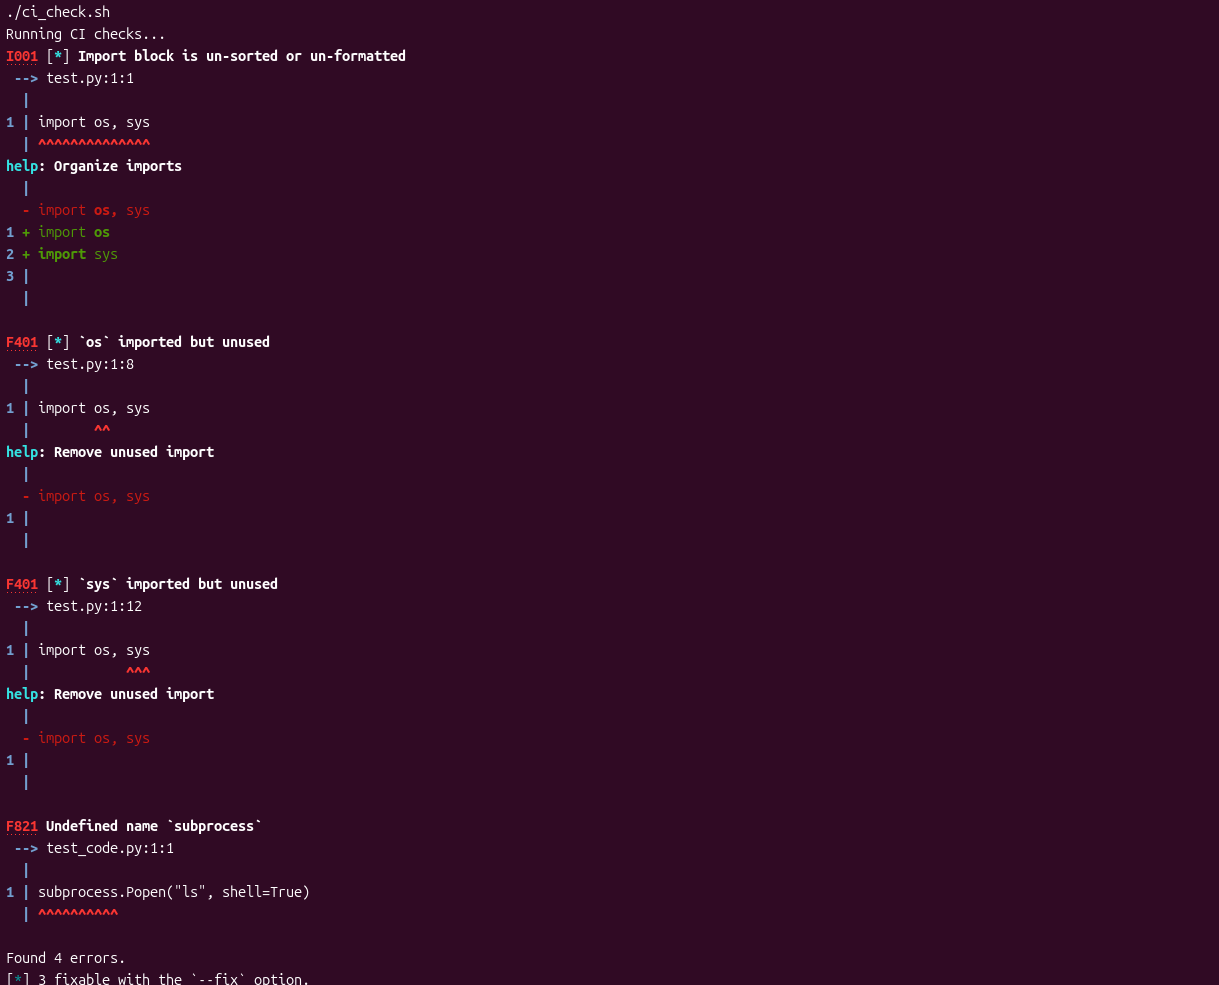
\includegraphics[width=0.9\textwidth]{ex10.jpg}
    \caption{实例10执行结果}
    \label{fig:ex10}
\end{figure}

\section*{三、解题感悟}

本次实验涵盖了代码质量工具、构建系统、API 数据处理和综合修复四个主题。

第13题让我把 ruff 和 pytest 集成到项目中，通过 check.sh 把格式化、检查、测试串成一条线，形成了本地质量门禁。第14题通过 Makefile 练习了增量构建，理解了依赖变化时只重建受影响产物的机制。第15题用 curl 和 jq 处理 API 数据，生成了 Markdown 报告，体验了命令行工具组合使用的便利。第16题模拟了一次完整的修复流程：从故意破坏代码、确认测试失败，到修复、构建 wheel 并计算 SHA-256。

课后10个实例练习了 ruff、pytest、pre-commit、sed、json 处理、Makefile、覆盖率测试等工具，这些在开发流程中都比较常用。整体来说，这一周的内容让我对代码质量保障和自动化构建有了更具体的认识。

\end{document}